
By way of guiding the user on how to best exploit the Parallel Patterns plugin, we will focus on the FaceDetect application \cite{FaceDetect}. The FaceDetect application uses an image-processing pipeline built on top of the PEPPHER framework. Within PEPPHER, pipeline patterns are expressed using annotated while-loops that comprise calls to multi-architectural components. The high-level FaceDetect code is shown in Figure \ref{fig:facedetect}. The application uses a four stage pipeline to perform detection of human faces on a stream of images. 

\definecolor{gray}{rgb}{0.9,0.9,0.9}
\definecolor{darkgreen}{rgb}{0.0,0.6,0.0}
\definecolor{codegreen}{RGB}{0,116,0}
\definecolor{codebrown}{RGB}{100,56,32}
\definecolor{codebackgroundcolor}{rgb}{0.933,0.925,0.882}
\definecolor{xmlelement}{RGB}{187,68,165}
\definecolor{xmlattr}{RGB}{0,0,0} %{167,125,58}
\definecolor{xmlval}{RGB}{207,49,37}
\lstset{
	frame=tb, 
    basicstyle=\scriptsize \ttfamily, 
    numberstyle=\footnotesize,
    showstringspaces=false,
    captionpos=b,
    breaklines=true, 
    language=c++,
    tabsize=2,
    xleftmargin=2em, framexleftmargin=2em, framextopmargin=0.5em, framexbottommargin=0.5em,  aboveskip=1.5em, belowskip=0.1em,  rulesepcolor=\color{gray}, abovecaptionskip=.5\baselineskip, belowcaptionskip=.1\baselineskip, backgroundcolor=\color{codebackgroundcolor}, escapechar=^
    }
    
The Parallel Patterns plugin for PTF supports automatic performance tuning of  high-level pipeline patterns built on top of the PEPPHER framework. The plugin searches for the best combination of pattern-specific parameters, parameters exposed by the runtime system, and machine-specific parameters such that execution is optimized for a given workload and target architecture.

The plugin for Parallel Patterns allows for the restriction of a potentially large search space via: 

  \begin{itemize}
    \item tuning range specifications for stage replication factors and stage buffer sizes by means of source code directives
    \item tuning range specifications for all tuning parameters via configuration file 
    \item performance analysis to focus tuning on the most time-consuming stage
  \end{itemize}

\begin{figure}[h]
\centering
\begin{lstlisting}
#pragma pph pipeline
while ( inputstream >> file ) {
    ReadImage ( file , image );
    ^\color{codebrown}{\#pragma pph stage replicate(?) buffer(?)}^
    ResizeAndColorConvert ( image, oimage );
    ^\color{codebrown}{\#pragma pph stage replicate(?) buffer(?)}^
    DetectFaces( oimage );
    WriteFaceDetectedImage ( file , oimage );
}
\end{lstlisting}
\caption{A pipeline pattern for face detection in a stream of images. The "?" symbols within the annotations indicate that the tuning ranges for \texttt{ResizeAndColorConvert} and \texttt{DetectFaces} stages should be automatically determined.}
\label{fig:facedetect}
\end{figure}

\subsubsection{Default behavior}

The total number of tuning scenarios in the search space is created as a crossproduct of the value ranges of all available tuning parameters. By default, for each of the tuning parameters the tuning range of possible values is determined by the system as follows:  

\begin{itemize}
\item for each stage replication factor that has been annotated with the "?" in the high-level code, the range of the stage replication factor is set to [1:(\textit{max\_execution\_units - number\_of\_pipeline\_stages - 1}):1]
\item for each buffer size, that has been annotated with the "?" in the high-level code, the range of the buffer size is set to [\textit{max\_execution\_units}:\textit{max\_execution\_units}*3:\textit{max\_execution\_units}]
\item the NCPUS range is set to [1:\textit{max\_cpu\_cores}:1]
\item the NGPUS range is set to [0:\textit{max\_gpus}:1]
\item {the SCHEDULING\_POLICY is set to two scheduling policies EAGER and HEFT\footnotemark}
\end{itemize}

These default values are based on the runtime system requirements and on the application testing experience. To minimize oversubscription, the total number of stages plus stage replicas is set to not exceed the number of execution units on the system. The buffer size influences the memory footprint of the application. For each stage, the buffer size is set to have minimum equal to the replication factor of that stage, and to have maximum of that value multiplied by 3.    

\footnotetext{HEFT (Heterogeneous Earliest Finish Time) considers inter-component data dependencies and schedules components to workers taking into account the current system load, available component implementation variants, and historical execution profiles, with the goal of minimizing overall execution time by favoring implementations variants with the lowest expected execution time. EAGER is a simply greedy scheduler. }

Tuning the pipeline on the system with many execution units may require an exploration of a huge search space. For instance, on the system with 16 CPU cores, and 4 GPUs, a full exhaustive search for the FaceDetect application would require an evaluation of 17*3*17*3*16*5*2 = 416,160 scenarios. In Table \ref{tab:fdfullspace} we summarize the possible values for each tuning parameter in this setup. 

\begin{table}[!h]
\begin{center}
\begin{tabular}{ @{} l @{} c }
\hline
\multicolumn{1}{c}{\textbf{ Tuning parameter }} & \textbf{ Possible values } \\
\hline
\hline
{ \texttt{ResizeAndColorConvert} Replication Factor}  & {1, 2, 3,.., 17} \\ \hline 
{ \texttt{ResizeAndColorConvert} Buffer Size} & {20, 40, 60}  \\ \hline  
{ \texttt{DetectFaces} Replication Factor}  &  {1, 2, 3,.., 17} \\ \hline 
{ \texttt{DetectFaces} Buffer Size} & {20, 40, 60} \\ \hline   
{ Number of CPU cores} & {1, 2, 3,.., 16} \\ \hline 
{ Number of GPUs} & {0, 1, 2, 3, 4} \\ \hline 
{ Scheduling Policy} & {``EAGER'', ``HEFT''}  \\ \hline 
\end{tabular}
\vspace{4pt}
\caption{Tuning parameters and their values on the PHIA system for the setup with no restrictions. }
\label{tab:fdfullspace}
\end{center}
\end{table}

The following three subsections demonstrate how to efficiently restrict the search space, and yet test majority of the performance-relevant scenarios. 
  
\subsubsection{Tuning range specification via directives}
The tuning range source code directives allow users to steer the tuning process of the plugin by specifying values for the stage replication factors and buffer sizes. 
Careful specification of the tuning ranges for such parameters in the high-level code may reduce the total number of scenarios that need to be tested.

For the FaceDetect application tuning, we used these directives to provide tuning ranges for the replication factors of the two middle stages in the pipeline. As shown in Figure \ref{fig:tuningrange}, the user specified tuning range starts with the minimum value of 1, which is incremented by 4 until it reaches the maximum value of 17, resulting in a total of 5 values for each tuning parameter. The minimum value of 1 will reveal if incrementing the replication factor for the certain stage has any effect on the performance. For the maximum value, it is usually good to keep the default of \textit{max\_execution\_units - number\_of\_pipeline\_stages - 1}. This will ensure that oversubscription is avoided. Finally, a good guideline for the increment is actual number of GPUs in the system, since the runtime system needs one CPU core for each GPU card it uses.   
 
\begin{figure}[htb]
\centering
\begin{lstlisting}
#pragma pph pipeline
while ( inputstream >> file ) {
    ReadImage ( file , image );
    ^\color{codebrown}{\#pragma pph stage replicate(1:17:4)}^
    ResizeAndColorConvert ( image, oimage );
    ^\color{codebrown}{\#pragma pph stage replicate(1:17:4)}^
    DetectFaces( oimage );
    WriteFaceDetectedImage ( file , oimage );
}
\end{lstlisting}
\caption{User-provided tuning hints. For the middle stages the tuning ranges for the stage replication factor is specified in  the form {\tt (min:max:step)}.}
\label{fig:tuningrange}
\end{figure}

By specifying tuning ranges for stage replication factors as shown in Figure \ref{fig:tuningrange}, the search space is reduced from 416,160 to 36,000 scenarios.

\subsubsection{Tuning range specification via configuration file}
Another option for enabling users to restrict the search space is by specifying tuning ranges in the SIR file for some or all tuning parameters (including NCPUS, NGPUS). 
In the configuration file, it is a good idea to provide tuning ranges for machine-specific tuning parameters, i.e., NCPUS and NGPUS. For instance, NCPUS parameter may be restricted in a way that the minimum number of CPU cores to be used for execution is equal to the number of pipeline stages, and the maximum is equal to the number of available CPU cores with an increment of 4 (see Figure \ref{fig:sirtuningrange}). As a consequence only 4 values for the NCPUS tuning parameter are considered, further restricting the search space to 9,000 scenarios. The tuning parameters and corresponding values that describe this restricted search space are summarized in Table \ref{tab:fdspaceretricted}.   

\begin{figure}[htb]
\centering
\begin{lstlisting}
...
  ^\color{xmlelement}{<selector}^ ^\color{xmlattr}{tuningActionType}^=^\color{xmlval}{"VAR"}^ ^\color{xmlattr}{tuningActionName}^=^\color{xmlval}{"NCPUS"}^ ^\color{xmlattr}{min}^=^\color{xmlval}{"4"}^ ^\color{xmlattr}{max}^=^\color{xmlval}{"16"}^ ^\color{xmlattr}{step}^=^\color{xmlval}{"4"}^^\color{xmlelement}{/>}^
...
 \end{lstlisting}
 \caption{In order to influence the tuning process\, the SIR file may be altered manually by changing the corresponding \textit{min}\, \textit{max} and \textit{step} values for the desired tuning parameter.}
 \label{fig:sirtuningrange}
\end{figure}

\begin{table}[!h]
\begin{center}
\begin{tabular}{ @{} l @{} c }
\hline
\multicolumn{1}{c}{\textbf{ Tuning parameter }} & \textbf{ Possible values } \\
\hline
\hline
{ \texttt{ResizeAndColorConvert} Replication Factor}  & {1, 5, 9, 13, 17} \\ \hline 
{ \texttt{ResizeAndColorConvert} Buffer Size} & {20, 40, 60}  \\ \hline  
{ \texttt{DetectFaces} Replication Factor}  & {1, 5, 9, 13, 17} \\ \hline 
{ \texttt{DetectFaces} Buffer Size} & {20, 40, 60}  \\ \hline   
{ Number of CPU cores} & {4, 8, 12, 16} \\ \hline 
{ Number of GPUs} & {0, 1, 2, 3, 4} \\ \hline 
{ Scheduling Policy} & {``EAGER'', ``HEFT''}  \\ \hline 
\end{tabular}
\vspace{4pt}
\caption{Tuning parameters and restricted values on the PHIA system.}
\label{tab:fdspaceretricted}
\end{center}
\end{table}

\subsubsection{Focused tuning via performance analysis}
Focused tuning of pipeline patterns via PTF pre-analysis may be enabled via \texttt{--vpattern-focused} command-line switch. In this mode, the plugin uses PTF's pre-analysis to detect the most performance-demanding stage in the pipeline. Once it has been detected, the tuning efforts are focused on the stage replication factor and buffer size of that stage. 

The focused tuning can be used without any additional user-provided hints. In the standalone mode it reduces the search space from initial 416,160 to 8,100. A combination of focused tuning with user-provided tuning ranges may be used to further decrease the search space. 
For the FaceDetect application the stage replication factor for the most performance-demanding stage (\texttt{DetectFaces}), is automatically set to [1:17:1], while for all other stages tuning of stage replication factors (and buffer sizes) is omitted.
As a result, the resulting scenario pool contains only 600 scenarios, significantly reduced from the initial total of 416,160 scenarios.  


Figure \ref{fig:bpg_comp} shows the effect of the different plugin features on the size of the search space. The first blue bar shows the number of scenarios when source code directives were used to restrict the search space from 416,160 to 36,000. The second blue bar represents additional restriction of the search space by adjusting tuning ranges directly in the configuration file. The third blue bar shows the number scenarios when only focused tuning via pre-analysis was used. Finally, the fourth blue bar shows the number of the scenarios when all features were used. 

\begin{figure}[h]
\centering
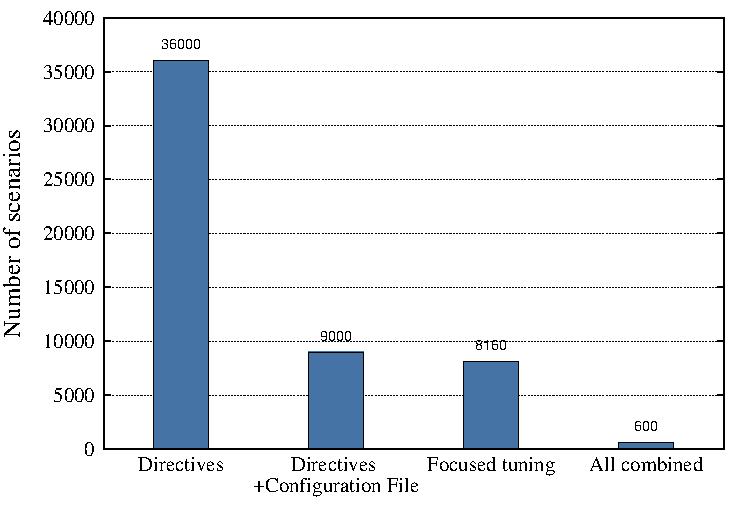
\includegraphics[width=14cm]{../BPG/phia-bpg.pdf}
\caption{Restricting the search space for the FaceDetect application using different plugin features of the Parallel Patterns plugin. }
\label{fig:bpg_comp}
\end{figure}

\subsubsection{Additional tips}
\begin{itemize} 
\item Stage Replication Factors

Stage replication factors determine the number of stage instances executed in parallel and therefore influence the degree of potential parallelism during application execution. Each stage replica will execute in an additional thread. To avoid oversubscription, the total number of stages plus stage replicas should not exceed the number of execution units on the system. On the other hand, if the replication factors are too low, the performance might be limited, so a good guideline is to increase stage replication factors for the stages that have higher performance demands. 
\item Machine-specific Parameters

The machine-specific parameters (NCPUS and NGPUS) are closely related to stage replication factors. The effective usage of system execution units may be hindered if the stage replication factors are not sufficiently high. On the other hand, if the total number of available execution units is small, the replication factor will have no effect. 

\end{itemize}


%\subsubsection{Plugin Features}

%The plugin for Parallel Patterns allows for the restriction of a potentially large search space 
%via:
%   \begin{itemize}
%    \item Tuning range specifications for stage replication factors and stage buffer sizes by means of source code directives: The tuning range source code directives allow users to steer the tuning process of the plugin by specifying values for the stage replication factors and buffer sizes. 
    %As shown in Figure \ref{fig:tuningrange}, the user specified tuning range starts with the minimum value of 1, which is incremented by 4 until it reaches the maximum value of 17, resulting in a total of 5 values for each tuning parameter. 
    
%    \item Tuning range specifications for all tuning parameters via configuration file: Restriction of the search space by specifying tuning ranges in the SIR file for some or all tuning parameters (including NCPUS, NGPUS).
    
%    \item Performance analysis to focus tuning on the most time-consuming stage: In this mode, the plugin uses PTF's pre-analysis to detect the most performance-demanding stage in the pipeline. Once it has been detected, the tuning efforts are focused on the stage replication factor and buffer size of that stage. 
   
%   \end{itemize}


%\subsubsection{Plugin Features}
%\begin{itemize}
%	\item Short description about the available tuning parameters
	
%The pipeline-specific tuning parameters target pipeline structural tuning parameters such as stage replication factors, and sizes of input/output buffers. Machine-specific parameters NCPUS and NGPUS are used to describe available hardware resources such as the number of available CPU cores (or available hardware threads) and number of usable graphic cards. Finally, the runtime-specific parameters include the scheduling policy used by the StarPU runtime system e.g., EAGER (simple greedy scheduler), HEFT (Heterogeneous earliest Finish Time), or similar.  

%The plugin supports follow tuning parameters: 
 %  \begin{itemize}
%	\item \emph{stage replication factor} - the number of stage instances that may be executed in parallel
%	\item \emph{sizes of buffers} - size of I/O buffers that hold data packets passed between pipeline stages
%	\item \emph{number of CPU cores} - number of available CPU cores to be used by the runtime system 
%	\item \emph{number of GPUs} - number of available graphic cards to be used for execution
%	\item \emph{scheduling strategy} - a scheduling policy used by StarPU runtime for scheduling component calls to available execution units of the target system
%   \end{itemize}

%The total number of tuning scenarios in the search space is created as a crossproduct of the value ranges of all available tuning parameters. 
%	\item Search Strategy
	
	
%	 The plugin for Parallel Patterns allows for the restriction of a potentially large search space via: 
	
%	\begin{itemize}	
%		\item If any other search strategy than exhaustive available.
%	\end{itemize}
	
%	\begin{itemize}
%		\item How to decide good replication factor or optimal resource count.
%		\item Selection of parameters to get optimal scenario quickly without exploding search space.
%	\end{itemize}
	
%	\item Use of SIR file to change the parameters
%	\begin{itemize}
%		\item Give range of values for a particular parameters
%	\end{itemize}

%	\item Choice of replication factor and its relation to the number of available resources
%	\begin{itemize}
%		\item Selecting higher replication factor than the resources for I/O, network abound tasks
%		\item How tuning parameters are used by the plugin and role of StarPU runtime. e.g. StarPU might decide to schedule tasks on CPU/GPU or both for some time even when replication factor is one.
%	\end{itemize}



%	\item Scheduling policy
%	\begin{itemize}
%		\item How to select appropriate scheduling policy.
%		\item HEFT uses historical data, how it improves over a period of time, how many runs it requires to see impact on execution time.
%	\end{itemize}
%	\item Buffer size
%	\begin{itemize}
%		\item In which cases buffer size plays important role
%		\item how to anticipate optimal buffer size
%	\end{itemize}
%\end{itemize}
